% !TEX root       = ./type_name.tex
% !TEX program    = pdflatex
% !TEX encoding   = utf-8
% !TEX spellcheck = de_DE_frami
%=======================================================================

%\chapter{Introduction}\label{ch:einleitung}
\chapter{Background}\label{ch:Background}
\sffamily{}

This chapter discusses about the topics relevant this thesis, it includes an introduction to software defined networking, 802.11 protocol, Hotspot 2.0 and BIC-IRAP project.

\section{Software Defined Networking \cite{SDN}}\label{sec:SDN}

SDN is nothing but the physical separation of the network control plane from the forwarding plane. The control plane consists of all the logic that the switch requires to correctly setup a forwarding plane, that is, the signaling associated with the switch.

Traditionally, the vendor has the control over the logic necessary for signaling since they run a proprietary firmware. This makes the devices non-interoperable with other vendors which hampers flexibility. Though most of these switches provide SNMP based management solution via CLI, they still do not allow the introduction of custom control plane function or protocol into the switch. This makes experimenting with new protocols cumbersome. Software Defines Networking aims to alleviate these problems by making the switched control plane be easily accessible remotely and be modifiable using the OpenFlow protocol. Any third-party software can than take advantage of this open protocol to manage and orchestrate an entire network.

SDN architecture generally has three components or groups of functionality as shown in the figure \ref{fig:sdn-architecture} below.

\begin{itemize}
	\item \textbf{Application Layer:}  Consists of programs that communicate the behaviors and needed resources with the SDN controller via the application protocol interfaces (API’s). It can also build an abstracted view of the network by collecting information from the controller.
	\item \textbf{Control Layer:} This logical layer functions as a relay that sends the instructions or resources sent by the application layer to the networking components.
	\item \textbf{Infrastructure Layer:} This holds the SDN networking devices that control the forwarding and data processing capabilities of the network including the function to forward and process the data paths.
\end{itemize}

\begin{figure}[H]
  \centering
  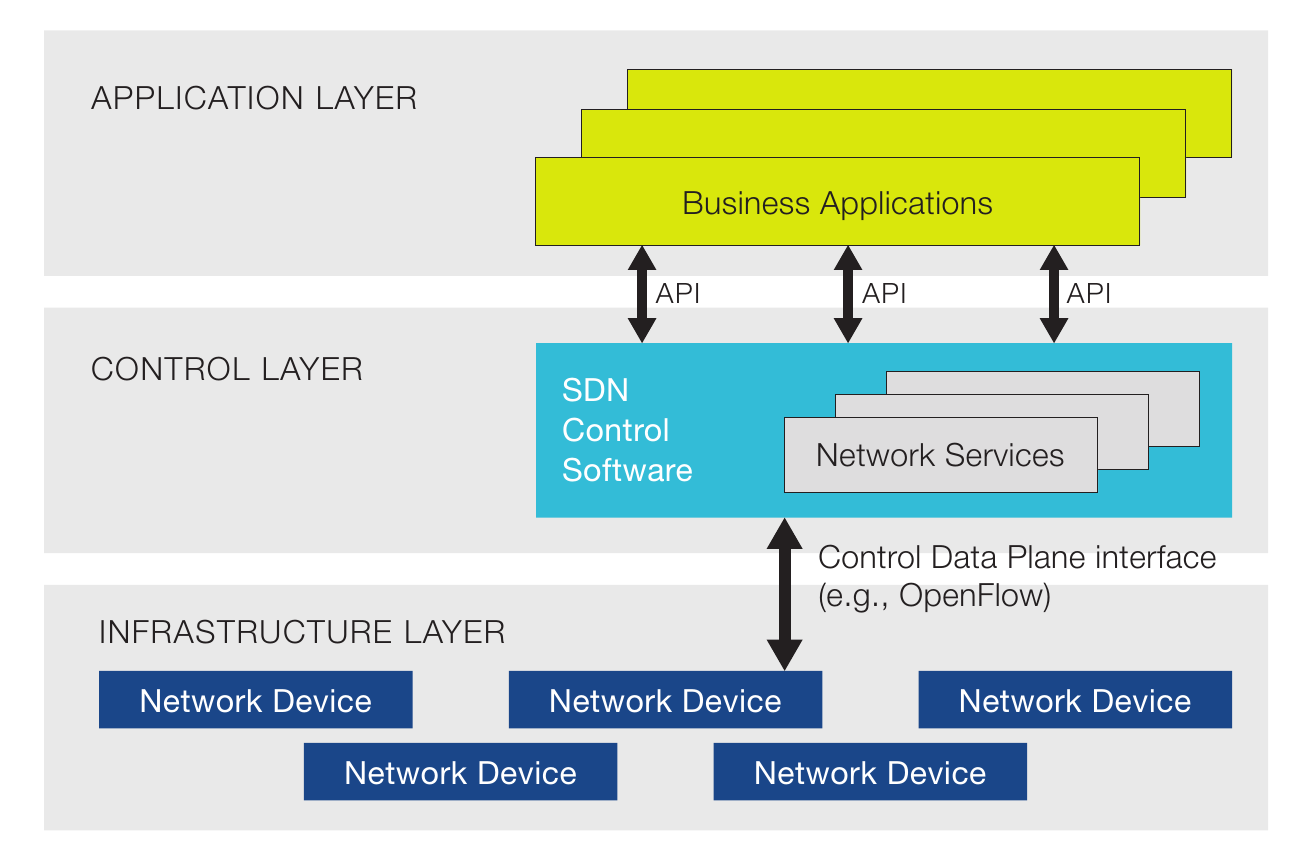
\includegraphics[width=1.0\linewidth]{sdn-architecture}
  \caption{SDN architecture diagram\cite{SDN:architecture}}
  \label{fig:sdn-architecture}
\end{figure}

\section{IEEE 802.11 MAC \cite{ieee2012802}}\label{sec:IEEE802.11}

The IEEE 802.11 Media Access Control Layer (MAC) \cite{ieee2012802} defines the protocol for stations
to establish connections with each other and transmit data frames.
Medium access in 802.11 is performed by a distributed coordination function (DCF), which uses carrier sense multiple access with collision avoidance (CSMA/CA) to enable random medium access among all contending stations (STAs). Hence, it reduces the amount of collisions. Logically, the MAC is divided into two parts, an upper MAC, and a lower MAC. The upper MAC handles management frames, which include probe, authentication, association requests and their corresponding responses. The lower MAC handles control frames, which includes acknowledgement (ACK) frames, along with request-to-send (RTS) and clear-to-send (CTS) frames. The frames handled by the lower MAC have real-time constraints. For instance, ACK frame timeouts are within the order of micro-seconds. For this reason, control frames are handled and generated within hardware. Management frames, however, have softer time constraints, and can be handled in software locally (as is the case in Linux systems that use hostapd \cite{hostapd}), or remotely (as is the case when using a centralized WLAN controller \cite{RFC5412L97} ).

An 802.11 based wireless interface can operate under the following operating modes: STA (client), access point (AP), mesh, ad-hoc and item Monitor mode. The most common mode of operation is the infrastructure mode (which includes enterprise WLAN environments). In this mode of operation, clients connect to the AP using a series of message exchanges in a process called “association”. The decision on which AP to associate with is left entirely to the client. Clients learn about APs either passively through beacon frames that are periodically broadcasted by the access points, or actively by performing a probe scan. 

In a probe scan, clients first send out probe request frames over all channels. APs that receive these frames and are willing to accept a connection from a client respond with a probe response frame. All APs from which the client receives probe responses are candidates for the client to associate with. Next, the client sends an authentication frame, and waits for an authentication response from the AP. This is followed by the client sending an association request, and receiving an association response from the AP. If the network is operating in open authentication mode, the client is considered to be
associated at this point, and can now transmit data frames to be forwarded by the AP. If the AP is configured to use WPA, WPA2, or WPA2 Enterprise, the corresponding 802.1X \cite{hostapd} handshake is performed after the association phase before clients can forward data frames through the AP.


\section{Hotspot 2.0 \cite{Hotspot_2.0_Definition}} \label{Hotspot2.0}

It is a new wireless network standard that is designed to make connection to public Wi-Fi hotspots more easy and secure. They are already supported on many mobile devices running some of the popular operating systems such as Windows 10, Mac OS 10.9 or newer, Android 6.0 or newer, and iOS 7 or newer.

The main purpose of Hotspot 2.0 is to provide seamless mobility like cellular style “roaming” for Wi-Fi networks. The device will automatically connect to the available networks based on the networks partners on the home networks while roaming globally. This is made possible using the latest 802.11u \cite{IEEE802.11u} protocol designed for the same purpose. Some organizations also call this as Passpoint \cite{Passpoint}.





%The technology behind OpenStack consists of a series of interrelated projects delivering various components for a cloud infrastructure solution. Each service provides an open API so that all of these resources can be managed through a dashboard that gives administrators control while empowering users to provision resources through a web interface, a command-line client, or software development kits that support the API.
%
%OpenStack is designed for horizontal scalability, so the user can easily add new compute, network, and storage resources to grow their cloud over time. In addition to the pervasiveness of massive OpenStack public clouds, many organizations, such as PayPal, Intel, and Comcast, build large-scale private clouds. OpenStack offers much more than a typical software package because it lets the user to integrate a number of different technologies to construct a cloud. This approach provides great flexibility, but the number of options might be daunting at first.
%
%OpenStack clouds are powered by various OpenStack projects.
%The selection of the components in openstack depends on how does the IaaS provider wants to use the OpenStack:
%
%\begin{figure}[H]
%  \centering
%  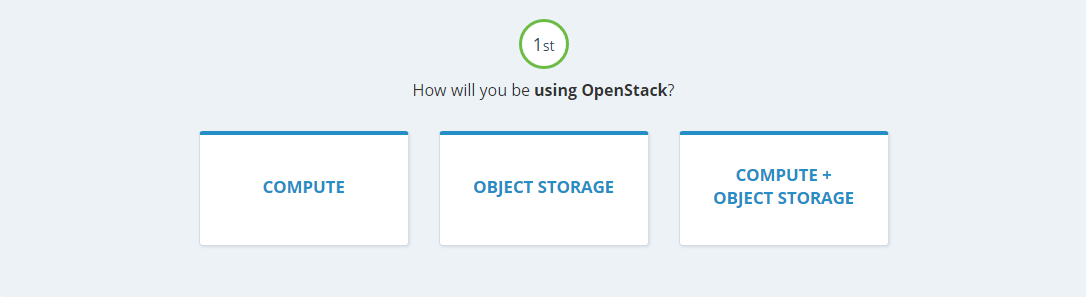
\includegraphics[width=1.0\linewidth]{Compute_ObjectStorage}
%  \caption{Primary objective to decide the purpose of having an OpenStack Cloud\cite{OpenStack}}\label{fig:Compute_ObjectStorage}
%\end{figure}
%
%The figure \ref{fig:Compute_ObjectStorage} actually specifies if the primary objective of the usage of OpenStack is, only with Compute - which defines the management of virtual machines on cloud, or only with Object Storage - which defines the allocation of end user based storage space on cloud, or the mix of both of Compute and Object Storage. Based on the objective of setting up the cloud, the core components can be selected as per the need from the wide range of available components.
%
%\section{Architecture of OpenStack}\label{sec:architecture}
%The OpenStack project is an open source cloud computing platform that aims for simple implementation, massive scalability, and a rich set of features. Cloud computing experts from around the world contribute to the project.
%
%OpenStack provides an Infrastructure-as-a-Service (IaaS) solution through a variety of complemental services. Each service offers an application programming interface (API) that facilitates this integration.
%
%\begin{figure}[H]
%	\begin{center}
%		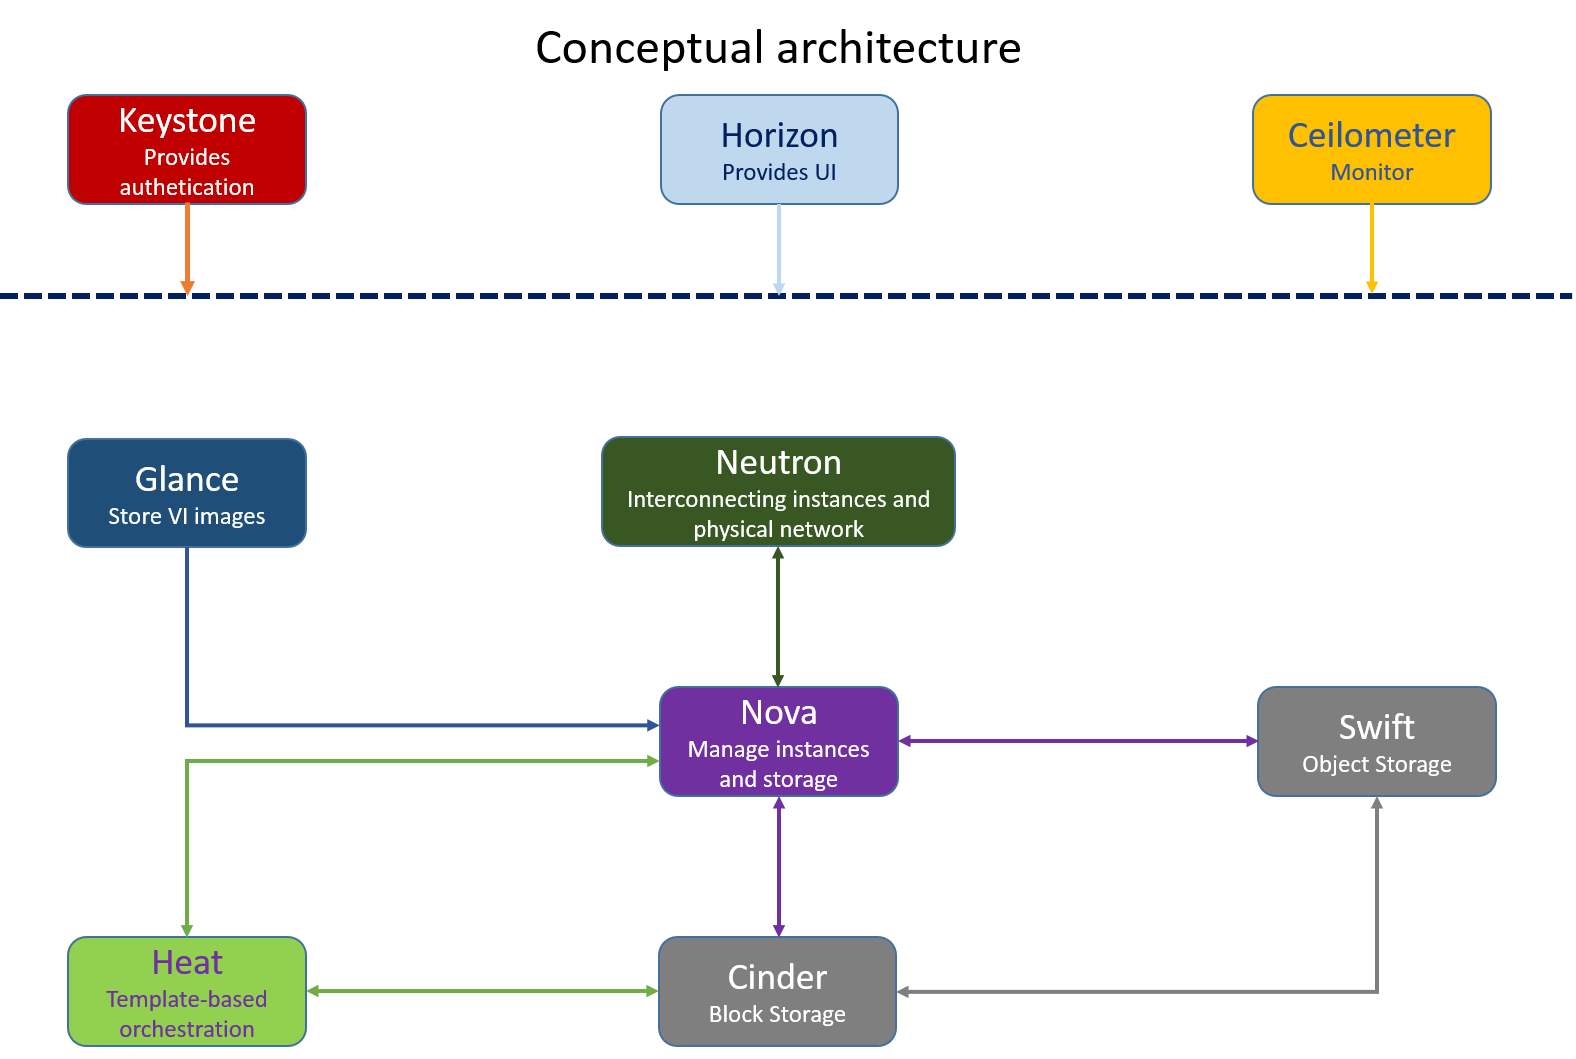
\includegraphics[width=1.0\linewidth]{conceptual_architecture}
%		\caption{The relationships among the OpenStack services}\label{fig:openstack_architecture}
%	\end{center}
%	\vspace{-10pt}
%\end{figure}
%
%The figure \ref{fig:openstack_architecture} shows the architecture of the services and how each service communicates with the other services and provide the desired cloud solution.
%
%The implementation of the services are based on the objective of having the OpenStack cloud.
%Each purpose of cloud solution have their own set of service requirements that needs to be installed on the nodes and enabled.
%
%\subsection{OpenStack for compute}\label{ssec:openstackforcompute}
%To set up the OpenStack for the purpose of Compute, it would require the implementation of the following services:
%\begin{itemize}
%  \item Identity service (Keystone) -- core service
%  \item Compute service (Nova) -- core service
%  \item Networking service (Neutron) -- core service
%  \item Block storage service (Cinder) -- core service
%  \item Image service (Glance) -- core service
%  \item Dashboard service (Horizon) -- optional
%  \item Telemetry service (Ceilometer) -- optional
%\end{itemize}
%
%\subsection{OpenStack for storage}\label{ssec:openstackforstorage}
%To set up the OpenStack for the purpose of storage, it would require the implementation of the following services:
%\begin{itemize}
%  \item Object storage service (Swift) -- core service
%  \item Identity service (Keystone) -- core service
%  \item Dashboard service (Horizon) -- optional
%  \item Telemetry service (Ceilometer) -- optional
%\end{itemize}
%
%
%\subsection{Description of the core services in OpenStack}\label{ssec:openstackservices}
%\begin{itemize}
%  \item Compute service (Nova) - Manages the lifecycle of compute instances in an OpenStack environment. Responsibilities include spawning, scheduling and decomissioning of machines on demand.
%  \item Object storage service (Swift) - Stores and retrieves arbitrary unstructured data objects via a RESTful, HTTP based API. It is highly fault tolerant with its data replication and scale out architecture. Its implementation is not like a file server with mountable directories.
%  \item Networking service (Neutron) - Enables network connectivity as a service for other OpenStack services, such as OpenStack Compute. Provides an API for users to define networks and the attachments into them. Has a pluggable architecture that supports many popular networking vendors and technologies.
%  \item Image service (Glance) - Stores and retrieves virtual machine disk images. OpenStack Compute makes use of this during instance provisioning.
%  \item Identity service (Keystone) - Provides an authentication and authorization service for other OpenStack services. Provides a catalog of endpoints for all OpenStack services.
%  \item Dashboard service (Horizon) - Provides a web-based self-service portal to interact with underlying OpenStack services, such as launching an instance, assigning IP addresses and configuring access controls.
%  
%  
%  \item Telemetry service (Ceilometer) - Monitors and meters the OpenStack cloud for billing, benchmarking, scalability, and statistical purposes.
%  \item Block storage service (Cinder) - Provides persistent block storage to running instances. Its pluggable driver architecture facilitates the creation and management of block storage devices.
%  \item Orchestration service (Heat) - Orchestrates multiple composite cloud applications by using either the native HOT template format or the AWS CloudFormation template format, through both an OpenStack-native REST API and a CloudFormation-compatible Query API.
%\end{itemize}
%
%The thesis is more focussed on the understanding of the nova compute service and the nova filter scheduler, and this would be documented further in the next sections the \nameref{sec:novacompute} and the \nameref{sec:novafilterschedulerdetailed}.
%
%\section{OpenStack Nova Compute}\label{sec:novacompute}
%Nova is an OpenStack project designed to provide power massively scalable, on demand, self service access to compute resources.
%Nova enables the lifecycle management of the virtual machines by provisioning or managing the resources for creation, management or deletion of virtual machines.
%
%Nova is further segregated into many sub modules based on the defined purpose like segregation of nodes, scheduling mechanism, management of virtual machines.
%
%\subsection{Host Aggregates}\label{ssec:hostaggregates}
%Nova enables the segregation of nova nodes by categorizing them into "Availability Zones" by the use of Host Aggregates mechanism.
%This mechanism helps to further divide resources based on Availability Zones. Host aggregates are visible only to the administrators whereas Availability zones are visible to the users. This information is used by the nova scheduler as to enable advanced scheduling or to define any logical groups for creation or migration of virtual machines.
%
%\subsection{Threading model}\label{ssec:threadingmodel}
%All OpenStack services use the green thread model of threading which reduces the likelihood of race conditions. In case of any code taking longer execution time and blocking any other threads for execution, an added eventlet code from the greenthread library will hlp to switch to process any pending threads.
%
%\subsection{Virtual Machine States and Transitions}\label{ssec:VirtualMachineStatesTransitions}
%Nova manages the state transitions of virtual machine throughtout the lifecycle from creation to deletion or handle any error states.
%When the creation of an instance is requested, the nova allocates the compute node for hosting the instance and enters the initial state of "building" and spawns the virtual instance unless there are any errors which would lead to the transition of the state to "error". As shown in \textit{Figure} \ref{fig:statetransitionsdiagram}, it provides the information about different transitional states along with the possible change of state instance state.
%
%\begin{figure}[H]
%	\begin{center}
%		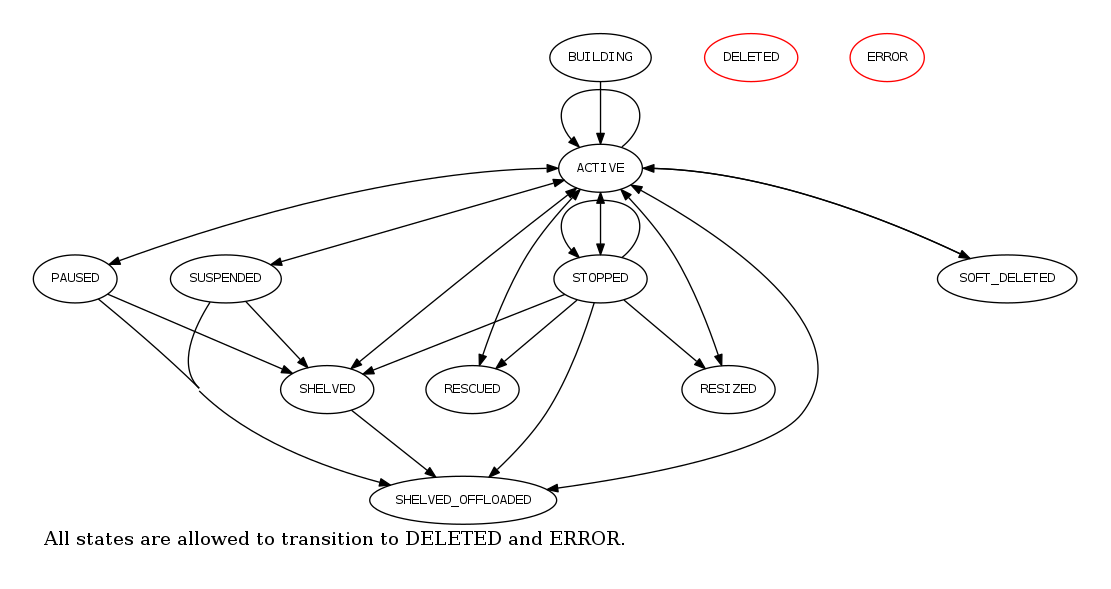
\includegraphics[width=1.0\linewidth]{state_transitions_diagram}
%		\caption{The diagram shows the allowed different state transistions of a virtual machine\cite{OpenStack:state_transitions}}\label{fig:statetransitionsdiagram}
%	\end{center}
%	\vspace{-10pt}
%\end{figure}
%
%\subsection{Filter Scheduler}\label{ssec:filterschedulermin}
%Nova has its own scheduling mechanism called "Filter Scheduler" which computes the placement decision of creation or migration of virtual instances.
%The scheduler is further explained in detail in the section \nameref{sec:novafilterschedulerdetailed}.
%
%\subsection{Advanced Message Queue Protocol and Nova}\label{ssec:amqpnova}
%The Advanced Message Queue Protocol (AMQP) is the messaging technology chosen by OpenStack to communicate between different nodes using a message queue enabler like RabbitMQ or Qpid.
%The nova components use the Remote Procedure Calls(RPC hereinafter) to communicate to one another. The RPC calls are authenticated for communication using message queue enabler like rabbitMQ, which validates the authentication using Keystone.
%
%\subsection{Block Device Mapping}\label{ssec:blockdevicemapping}
%Nova has a concept of block devices that can be exposed to cloud instances.
%Block device mapping is a way to organize and keep data about all of the block devices an instance has.
%
%\subsection{Nova OpenStack RESTful API}\label{ssec:novarestapi}
%The Nova provides the RESTful API which is exposed as an HTTP request service for routing, controllers and actions, serialization and trigering faults.
%
%\subsection{Conductor}\label{ssec:novaconductor}
%Conductor serves as a database proxy, object backporter and also as a centralized place to manage the execution of workflows which involve the scheduler.
%
%\subsection{Notifications in Nova}\label{ssec:novanotifications}
%Similarly to other OpenStack services Nova emits notifications to the message bus with the Notifier class provided by oslo.messaging.
%
%\section{Standard Nova Filter Scheduler}\label{sec:novafilterschedulerdetailed}
%The \textbf{Filter Scheduler} supports filtering and weighting to make informed decisions on where a new instance should be created.
%This Scheduler supports working with Compute Nodes only.
%\begin{figure}[H]
%	\begin{center}
%		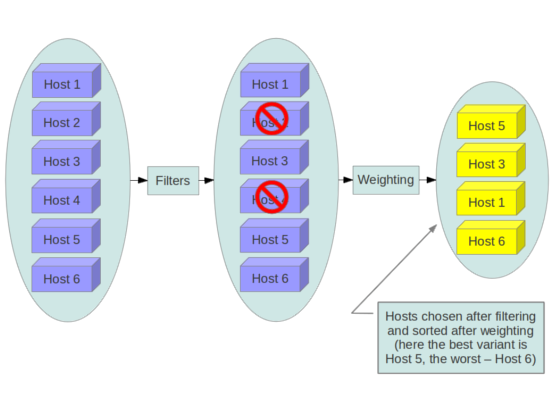
\includegraphics[width=1\linewidth]{filteringWorkflow1}
%		\caption{Filtering the compute hosts and sorting them based on weights\cite{OpenStack:filteringworkflow1}}\label{fig:filteringWorkflow1}
%	\end{center}
%	\vspace{-10pt}
%\end{figure}
%The filter scheduler iterates over all the available compute nodes, evaluates each compute node against the set of filters, and a list of the possible nodes for instance creation is generated sorted based on the weights.
%The scheduler then chooses the best host for the instance by choosing the most weighted host. For any specific filter to pass a specific host, the filter matches the users request against the state of the host as defined by each filter definition.
%
%If the scheduler does not find any hosts and returns an empty set of list of hosts for any requested instance, it means that there is no possible host where the instance can be placed to complete the user request.
%
%The filter scheduler has to be flexible to support the required variety of filtering and weighting strategies. The nova also permits to implement the user's own filtering algorithm.
%
%\subsection{Filtering}\label{ssec:novafiltering}
%There are many standard filter classes which may be used (nova.scheduler.filters):
%\begin{itemize}
%    \item \textbf{AllHostsFilter} - The initial hosts filter to pass all the available hosts.
%
%    \item \textbf{ImagePropertiesFilter} - This filters the possible hosts based on properties defined by the instance's image. It passes hosts that can support the properties specified on the image used by the instance.
%
%    \item \textbf{AvailabilityZoneFilter} - This filters the hosts which are grouped by availability zone. It passes only those hosts which match the availability zone specified in the instance properties.
%
%    \item \textbf{ComputeCapabilitiesFilter} - This filter checks that if the capabilities provided by the host compute service satisfy any extra specifications associated with the instance type. It passes hosts that can create the specified instance type.
%
%    \item \textbf{ComputeFilter} - This passes all the hosts that are operational and enabled.
%
%    \item \textbf{CoreFilter} - This filters the hosts based on available VCPU cores. It passes hosts with sufficient number of CPU cores.
%
%    \item \textbf{AggregateCoreFilter} - This filters the hosts by CPU core number with \\per-aggregate \verb|cpu_allocation_ratio| setting specified in the nova configuration. If no per-aggregate value is found, it will fall back to the global default \verb|cpu_allocation_ratio|.
%
%    \item \textbf{IsolatedHostsFilter} - This filter is based on \verb|image_isolated|, \verb|host_isolated| and \verb|restrict_isolated_hosts_to_isolated_images| flags.
%
%    \item \textbf{JsonFilter} - This filter allows simple JSON-based grammar for selecting hosts.
%
%    \item \textbf{RamFilter} - This filters the hosts by their available RAM capacity. Only those hosts with sufficient RAM capacity to host the instance are passed.
%
%    \item \textbf{AggregateRamFilter} - This filters the hosts by RAM with per-aggregate \\\verb|ram_allocation_ratio| setting specified in the nova configuration. If no per-aggregate value is found, it will fall back to the global default \\\verb|ram_allocation_ratio|. 
%
%    \item \textbf{DiskFilter} - This filters the hosts by their storage space. Only hosts with sufficient storage space to host the instance are passed.
%
%    \item \textbf{AggregateDiskFilter} - This filters the hosts by disk allocation with per-aggregate \verb|disk_allocation_ratio| setting. If no per-aggregate value is found, it will fall back to the global default \verb|disk_allocation_ratio|.
%
%    \item \textbf{NumInstancesFilter} - This filters the compute nodes by number of running instances. Nodes with too many instances will be filtered out.
%
%    \item \textbf{AggregateNumInstancesFilter} - This filters the hosts by number of instances with per-aggregate \verb|max_instances_per_host| setting.
%
%    \item \textbf{IoOpsFilter} - This filters the hosts by concurrent I/O operations on it. The hosts with too many concurrent I/O operations will be filtered out.
%
%    \item \textbf{AggregateIoOpsFilter} - filters hosts by I/O operations with per-aggregate \verb|max_io_ops_per_host| setting. If no per-aggregate value is found, it will fall back to the global default \verb|max_io_ops_per_host|.
%
%    \item \textbf{PciPassthroughFilter} - This filter schedules instances on a host if the host has devices to meet the device requests in the \verb|‘extra_specs’| for the flavor.
%
%    \item \textbf{SimpleCIDRAffinityFilter} - This filter allows a new instance on a host within the same IP block.
%
%    \item \textbf{DifferentHostFilter} - This filter allows the instance on a different host from a set of instances.
%
%    \item \textbf{SameHostFilter} - This filter puts the instance on the same host as another instance in a set of instances.
%
%    \item \textbf{RetryFilter} - This filters the hosts that have been attempted for scheduling. Only passes hosts that have not been previously attempted.
%
%    \item \textbf{TrustedFilter} (EXPERIMENTAL) - This filters the hosts based on their trust. Only passes hosts that meet the trust requirements specified in the instance properties.
%
%    \item \textbf{TypeAffinityFilter} - Only the hosts that are not already running an instance of the requested type are passed.
%
%    \item \textbf{AggregateTypeAffinityFilter} - This limits \verb|instance_type| by aggregate.
%
%    \item \textbf{ServerGroupAntiAffinityFilter} - This filter implements anti-affinity for a server group.
%
%    \item \textbf{ServerGroupAffinityFilter} - This filter works the same way as ServerGroupAntiAffinityFilter. The difference is that when you create the server group, you should specify a policy of ‘affinity’.
%
%    \item \textbf{AggregateMultiTenancyIsolation} - This isolate the tenants in specific aggregates.
%
%    \item \textbf{AggregateImagePropertiesIsolation} - This isolates the hosts based on image properties and aggregate metadata.
%
%    \item \textbf{MetricsFilter} - This filters the hosts based on metrics \verb|weight_setting|. Only those hosts with the available metrics are passed.
%
%    \item \textbf{NUMATopologyFilter} - This filters the hosts based on the NUMA topology requested by the instance, if any.
%\end{itemize}
%
%\subsection{Weights}\label{ssec:novaweights}
%Filter Scheduler uses the weight based approach during its selection of a host for the requested instance.
%A weigher is a way to select the best suitable host from a group of valid hosts by giving weights to all the hosts in the list.
%
%In order to prioritize one weigher against another, all the weighers have to define a multiplier that will be applied before computing the weight for a node. All the weights are normalized beforehand so that the multiplier can be applied easily. Therefore the final weight for the object will be:
%\begin{lstlisting}[frame=single]
%weight = w1_multiplier * norm(w1) + w2_multiplier * norm(w2) + ...
%\end{lstlisting}
%
%The Filter Scheduler weighs hosts based on the config option \verb|scheduler_weight_|- \verb|classes|, this defaults to \verb|nova.scheduler.weights.all_weighers|, which selects the following weighers:
%
%\begin{itemize}
%	\item \textbf{RAMWeigher} - Compute weight based on available RAM on the compute node.
%
%	\item \textbf{DiskWeigher} - Hosts are weighted and sorted by free disk space with the largest weight winning.
%
%	\item \textbf{MetricsWeigher} - This weigher can compute the weight based on the compute node host’s various metrics.
%		The to-be weighed metrics and their weighing ratio are specified in the configuration file as the followings:
%\begin{lstlisting}[frame=single]
%metrics_weight_setting = name1=1.0, name2=-1.0
%\end{lstlisting}
%
%	\item \textbf{IoOpsWeigher} - The weigher can compute the weight based on the compute node host’s workload. The default is to preferably choose light workload compute hosts.
%
%	\item \textbf{ServerGroupSoftAffinityWeigher} - The weigher can compute the weight based on the number of instances that run on the same server group.
%		The largest weight defines the preferred host for the new instance.
%
%	\item \textbf{ServerGroupSoftAntiAffinityWeigher} - The weigher can compute the weight based on the number of instances that run on the same server group as a negative value.
%
%	\item \textbf{IoOpsWeigher} - Hosts are weighted and sorted by free disk space with the largest weight winning.
%\end{itemize}
%
%Filter Scheduler makes a local list of acceptable hosts by repeated filtering and weighing.
%Each time it chooses a host, it virtually consumes resources on it, so subsequent selections can adjust accordingly.
%It is useful if the customer asks for a large block of instances, because weight is computed for each instance requested.
%
%\begin{figure}[H]
%	\begin{center}
%		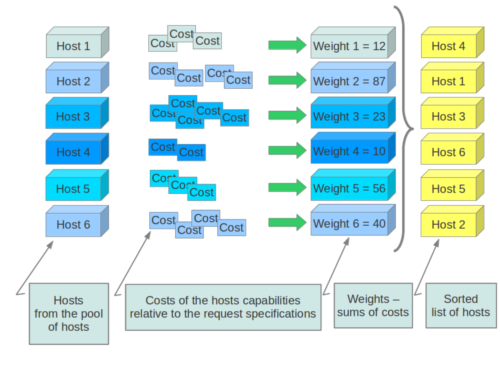
\includegraphics[width=1\linewidth]{filteringWorkflow2}
%		\caption{Compute hosts sorted based on weights\cite{OpenStack:filteringWorkflow2}}\label{fig:filteringWorkflow2}
%	\end{center}
%	\vspace{-10pt}
%\end{figure}
%
%At the end, the Filter Scheduler sorts selected hosts by their weight and attempts to provision instances on the chosen hosts.
%
%\section{Opening for any improvements in the filter scheduler?}\label{sec:openingforimprovement}
%The filter scheduler executes the instances one instance at a time.
%If an user requests for bulk creation of instances, for example: consider a request for creation of \verb|n| instances, the filter scheduler would need to run for \verb|n| number of times to execute the placement decision for each requested instance.
%
%If the user's request for the creation of large number of instances could be modelled into a Linear programming model with the parameters that are required to filter the hosts and then computing them into a Linear programming solver like cPlex, the resultant solution could achieve better results with lesser execution time for the creation of large number of instances.
%
%There could be many possibilities of modelling the linear programming model to have a placement decision of the host like the Virtual Network Embedding problem.
%Such problems are also known as knapsack problem in combinatorial optimisation.
%
%Given the current availability of input data, there is also no possibility of network aware scheduling which would consider the amount of network load on the host machines before placing the instance.
%
%With the learning curve of OpenStack, there could be many possibilities to optimise and solve the instance scheduling problem based on the purpose of the cloud provider and the availability of the inputs to model the Linear program with a better scheduling approach.
%
%\section{Structure of the thesis}\label{sec:thesisstructure}
%The first chapter \nameref{ch:introduction_cloud} provides the basic concept of cloud and its offerings. This chapter \nameref{ch:introduction_openstack} gives an idea about OpenStack as an IaaS model and the brief understanding about the services offered by OpenStack.
%
%The next chapter \nameref{ch:installationofopenstack} will explain the implementation of the services to set up the OpenStack for the purpose of computing.
%The chapter \nameref{ch:novaalgorithm} would explain about the Nova Filter Scheduler and the flow of code as how the filter scheduler algorithm is invoked during creation of instances.
%Then the chapter \nameref{ch:implementationofcplex} would explain the new mathematical formulation used to schedule the instances and its implementation.
%In the chapter \nameref{ch:comparisionofbothscheduler} one could see and evaluate the performance between the existing filter scheduler and the new modelled scheduler algorithm followed by the chapters \nameref{ch:futurepossibilities} and \nameref{ch:Conclusion}.


%Auch zeigt \ref{fig:bildtbd}, dass es genau so ist. Man könnte das auch mit einer \gls{gls:app}
%realisieren. \missing{Quelle des Bildes noch ergänzen.}